%% Version 0.001 of Poly PhD thesis template.
%% Time-stamp: <2011-12-27 14:52:09 Boris Aronov>

\documentclass[letterpaper]{polythesis} 

%% This controls the sizes, spacing, and font of section headings.  It
%% does NOT control the layout of chapter header pages.  There are
%% many different styles possible.
\usepackage[medium]{titlesec}

% Allows box rotation.  Uncomment if you need it.
% \usepackage{rotate}

%% Using CMR fonts.  Add appropriate font commands if you want to
%% switch to something else.  Be warned that there are virtually zero
%% text/math font combinations available that work well in TeX.  It's
%% a standard TeX FAQ

\usepackage{calc}

%% Occasionally needed for weird footnote behavior  Do not use if you
%% have no footnotes in your thesis.
%\usepackage[bottom]{footmisc}

%% WARNING:  This will BREAK if your subfigure.sty is v2.0 or before!
\usepackage[subfigure]{ccaption}
\usepackage{subfigure}

%\usepackage{type1cm}
\usepackage{url, cite, graphicx, algorithmic, amsmath, amsfonts, amsthm}
\usepackage[chapter]{algorithm}

%% this is a customized package
%% Do NOT use unless you ABSOLUTELY have to.  Nesting sections that
%% deep is ridiculous.
% \usepackage{subsections}
% \setcounter{secnumdepth}{5}
% \setcounter{tocdepth}{5}

%% Abbreviations that you might need...
% \newcommand{\AA}{\mathcal{A}}
% \newcommand{\reals}{\mathbb{R}}
% ...

\newtheorem{condition}{Condition}[section]
\newtheorem{definition}{Definition}[section]
\newtheorem{theorem}{Theorem}[section]
\newtheorem{lemma}[theorem]{Lemma}
\newtheorem{cor}[theorem]{Corollary}
\newtheorem{corollary}[theorem]{Corollary}
\newtheorem{claim}[theorem]{Claim}
\newtheorem{fact}[theorem]{Fact}
\newtheorem{example}[section]{Example}
\newtheorem{note}{Note}[section]

%% Some trickery to be able to add stuff in before the first chapter.
\def\nonumchapter#1{%
    \chapter*{#1}
    \addcontentsline{toc}{chapter}{#1}}

\def\prefacesection#1{%
    \chapter*{#1}
    \addcontentsline{toc}{chapter}{#1}}

\def\afterpreface{\newpage
    \pagenumbering{arabic}
    \typeout{Thesis preface pages completed.}
    }

%% New operators if you need them.
% \DeclareMathOperator{\area}{area}

%% Uncomment if you need to see every file your document uses, with
%% all versions.
% \listfiles

\begin{document}

\frontmatter

\title{Fancy Research Results of World-Wide Importance}
\author{Generic M.\ Student}

\date{\today}

\pagenumbering{roman}

\maketitle

{\setstretch{2}
% $Id: title.tex,v 1.1 2003/08/26 22:53:19 Administrator Exp Administrator $
\thispagestyle{empty}
\begin{center}
{\large
%% Title
{\bf FANCY RESEARCH RESULTS OF WORLD-WIDE IMPORTANCE}\\
\mbox{} \\
{\huge \bf DISSERTATION}\\
\mbox{} \\
Submitted in Partial Fulfillment\\
of the Requirements for the\\
Degree of\\
{\bf DOCTOR OF PHILOSOPHY (Computer Science)}\\
at the\\
{\bf NEW YORK UNIVERSITY\\POLYTECHNIC SCHOOL OF ENGINEERING}\\
by\\
{\bf Generic M.\ Student}\\
\mbox{} \\
% The date appearing on the title page should be the month and year of
% the expected degree award (e.g., January 20XX or May/June 20XX) 
% and not the completion date of the work.
{\bf Month 20xx}}
\end{center}
\vspace{.35 in}
\hspace{4 in} Approved:

\vspace{.2 in}

\hspace{3.35 in} \hrulefill\

\vspace{-.2 in}

\hspace{3.6 in} Department Head

\vspace{.2 in}

\hspace{-.5 in}Copy No. \hrulefill\ \hspace{4 in}

\vspace{-.4 in}

\hspace{3.35 in} \hrulefill\ %\hspace{.5 in}

%\vspace{-.39 in}

%\hspace{4.8 in} , 20\hrulefill\

%% Rules seem to say all page numbers except for the title page have a number.
%\thispagestyle{empty}
\thispagestyle{plain}
\mbox{} \\
{\large
Approved by the Guidance Committee :

\vspace{.2 in}

\hspace{.2 in} \underline{Major} : Computer Science

\vspace{.2 in plus 1fill}

\hspace{3.2 in} \hrulefill\

\vspace{-.2 in}

\hspace{3.2 in} Ver E.\ Important
\vspace{-.1 in}

\hspace{3.2 in} Professor of

\vspace{-.2 in}

\hspace{3.2 in} Computer Science

\vspace{.2 in plus 1fill}




\hspace{3.2 in} \hrulefill\

\vspace{-.2 in}

\hspace{3.2 in} Snob Ish Prof
\vspace{-.1 in}

\hspace{3.2 in} Assistant Professor of

\vspace{-.2 in}

\hspace{3.2 in} Computer \& Information Science

\vspace{.2 in plus 1fill}

\hspace{3.2 in} \hrulefill\

\vspace{-.2 in}

\hspace{3.2 in} Doctor D. Doctor
\vspace{-.1 in}

\hspace{3.2 in} Associatte Professor of

\vspace{-.2 in}

\hspace{3.2 in} Creative Data Manipulation

%% No more Minors in CS!
% \vspace{.2 in}

% \hspace{.2 in} \underline{Minor} : Atmospheric Science

\vspace{.2 in plus 1fill}

\hspace{3.2 in} \hrulefill\

\vspace{-.2 in}

\hspace{3.2 in} Thomas (Breezy) Windmill
\vspace{-.1 in}

\hspace{3.2 in} Professor of
\vspace{-.2 in}

\hspace{3.2 in} Atmospheric Science

\vspace{0 in plus 1fill}

}
}
% Rules seem to say: Number everything except for titlepage.
%\thispagestyle{empty}
\thispagestyle{plain}
\begin{center}
\vspace{2in}
{\large
Microfilm or copies of this dissertation may be obtained from}
\vspace{3in}

{\large
UMI Dissertation Publishing\\
ProQuest CSA\\
789 E. Eisenhower Parkway\\
P.O. Box 1346\\
Ann Arbor, MI 48106-1346}
\end{center}

\prefacesection{Vita}

%% From the rules:
% Give date and place of birth and a brief educational and
% professional history.  Clearly state period of time devoted to the
% research or project, the laboratories in which it was performed, and
% the source of any special support (research contract, research
% grant, fellowship, assistantship, traineeship, etc.). A vita page is
% NOT the same thing as a resume.

Generic M.\ Student was born in ... 
She received her ABCD degree in Financial Machinations from the ZYX
School of Advanced Manipulation, in Big City, Far Away Country.
She received her ...

\newenvironment{dedication}
  {\cleardoublepage 
   %% Rules seem to say dedication page should have a page number
   % \thispagestyle{empty} 
   \thispagestyle{plain} 
   \vspace*{\stretch{1}} \begin{center} \em}
  {\end{center} \vspace*{\stretch{3}} \clearpage}
\begin{dedication}

To my favorite poodle, Snow White.

\end{dedication}
 %% OPTIONAL
% Thesis Acknowledgements ----------------------------------------------
\prefacesection{Acknowledgements}

I would like to thank Professor XXX for this and that.  I would also
like to mention my friends, and my family, and, last but not least, my
noisy next-door neighbor Skunk without whose ``help'' this thesis would have
been finished five years earlier.

\bigskip\medskip

\noindent \hfill Generic M.\ Student, New York University Polytechnic School of Engineering

\hfill \today

% ----------------------------------------------------------------------
 %% OPTIONAL

\vspace*{3ex plus 0.6fil}
\begin{center}
\addcontentsline{toc}{chapter}{Abstract}

{\large\bf
   AN ABSTRACT\\[3ex]
%% Title
   FANCY RESEARCH RESULTS OF WORLD-WIDE IMPORTANCE\\[2ex]
   by\\[3ex]
   Generic M.\ Student\\[3ex]
   %% Advisor name
   Advisor: Ver E.\ Important\\[2ex]
   %% Co-advisor, or comment out
   Co-Advisor: NAME, IF THERE IS A CO-ADVISOR
}\\[3ex]
Submitted in Partial Fulfillment of the Requirements\\[2ex]
for the Degree of Doctor of Philosophy (Computer Science)\\[3ex]
% The date appearing on the title page should be the month and year of
% the expected degree award (e.g., January 20XX or May/June 20XX) 
% and not the completion date of the work.
Month 20xx
\end{center}

\vspace*{2.5ex}

The problem of \emph{fuzzy guzzles} arises in numerous areas of human
endeavor.  In this thesis we address ...

text text text text text text text some text some text some text some
text some text some text some text some text some text some textsome
text some text some text some text some text some text some text some
text some text some textsome text some text some text some text some
text some text some text some text some text some textsome text some
text some text some text some text some text some text some text some
text some textsome text some text some text some text some text some
text some text some text some text some text

\vspace*{3ex plus 1fil}
\tableofcontents
%% Comment out appropriate lines below if you have no figures, or no
%% tables, or no algorithms.
%% Rules say that if you have 10 or fewer figures you need not include
%% the list of tables.  Same with figures.
\listoffigures 
\listoftables
\listofalgorithms

\afterpreface

\mainmatter

%%% ------------- uncomment the following line to enable true double spacing
%\doublespacing
% This is for 1 1/2 spacing, which is usually good enough. Comment
% this out if you want really double spaceing.
\onehalfspacing

%% Chapter 1
\chapter{Introduction}
\label{chap:intro}

Here is the introduction of my beautiful thesis.  I will give some
history, summarize other people's work, and finally explain what I did
in the thesis.  Isn't it great?  It has even been cited already
once~\cite{xxxx}.

Here are some possible sections to put into your thesis...

\section{Motivation}
\label{sec:motivation}

some text some text some text some text some text some text some text
some text some text some textsome text some text some text some text
some text some text some text some text some text some textsome text
some text some text some text some text some text some text some text
some text some textsome text some text some text some text some text
some text some text some text some text some textsome text some text
some text some text some text some text some text some text some text
some text

\section{History and previous research}
\label{sec:history}

some text some text some text some text some text some text some text
some text some text some textsome text some text some text some text
some text some text some text some text some text some textsome text
some text some text some text some text some text some text some text
some text some textsome text some text some text some text some text
some text some text some text some text some textsome text some text
some text some text some text some text some text some text some text
some text

\section{Our contributions}
\label{sec:contribution}

some text some text some text some text some text some text some text
some text some text some textsome text some text some text some text
some text some text some text some text some text some textsome text
some text some text some text some text some text some text some text
some text some textsome text some text some text some text some text
some text some text some text some text some textsome text some text
some text some text some text some text some text some text some text
some text

\section{Organization of the thesis}
\label{sec:organization}

some text some text some text some text some text some text some text
some text some text some textsome text some text some text some text
some text some text some text some text some text some textsome text
some text some text some text some text some text some text some text
\begin{figure}
  \centering
  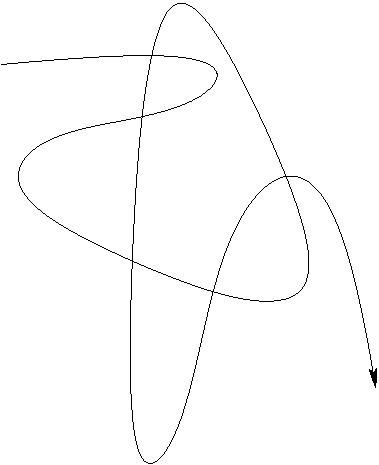
\includegraphics[width=0.3\textwidth]{chapter1/org}
  \caption{The organization of this thesis}
  \label{fig:organization-1}
\end{figure}
some text some textsome text some text some text some text some text
some text some text some text some text some textsome text some text
some text some text some text some text some text some text some text
some text


\chapter{Second Chapter}
\label{chap:second}

In this chapter we finally get to the technical subject of this
thesis...

some text some text some text some text some text some text some text
some text some text some textsome text some text some text some text
some text some text some text some text some text some textsome text
some text some text some text some text some text some text some text
some text some textsome text some text some text some text some text
some text some text some text some text some textsome text some text
some text some text some text some text some text some text some text
some text

\section{Standard definitions and background}
\label{sec:definitions}

some text some text some text some text some text some text some text
some text some text some textsome text some text some text some text
some text some text some text some text some text some textsome text
some text some text some text some text some text some text some text
some text some textsome text some text some text some text some text
some text some text some text some text some textsome text some text
some text some text some text some text some text some text some text
some text

\section{The notion of a Googly Booze Fiddle}
\label{sec:notion}

We finally introduce the \emph{Googly Booze Fiddle}, which is at the
heart of our revolutional new contribution to Computer Science...

some text some text some text some text some text some text some text
some text some text some textsome text some text some text some text
some text some text some text some text some text some textsome text
some text some text some text some text some text some text some text
some text some textsome text some text some text some text some text
some text some text some text some text some textsome text some text
some text some text some text some text some text some text some text
some text

%% Here's a section that's in a separte file...
\section{Discussion}
\label{sec:discussion}

some text some text some text some text some text some text some text
some text some text some textsome text some text some text some text
some text some text some text some text some text some textsome text
some text some text some text some text some text some text some text
some text some textsome text some text some text some text some text
some text some text some text some text some textsome text some text
some text some text some text some text some text some text some text
some text



\chapter{Some Other Chapter}
\label{chap:other}

In this chapter we first describe 

some text some text some text some text some text some text some text
some text some text some textsome text some text some text some text
some text some text some text some text some text some textsome text
some text some text some text some text some text some text some text
some text some textsome text some text some text some text some text
some text some text some text some text some textsome text some text
some text some text some text some text some text some text some text
some text

\section{Another section...}
\label{sec:92183}

some text some text some text some text some text some text some text
some text some text some textsome text some text some text some text
some text some text some text some text some text some textsome text
some text some text some text some text some text some text some text
some text some textsome text some text some text some text some text
some text some text some text some text some textsome text some text
some text some text some text some text some text some text some text
some text

%% another section that lives in a separate file...
\section{One of infinitely many sections...}
\label{sec:one-of-many}

some text some text some text some text some text some text some text
some text some text some textsome text some text some text some text
some text some text some text some text some text some textsome text
some text some text some text some text some text some text some text
some text some textsome text some text some text some text some text
some text some text some text some text some textsome text some text
some text some text some text some text some text some text some text
some text




\bibliographystyle{plain}
{\singlespace
%% If you are using BibTeX, else comment out
\bibliography{bibliography}
%% If you are not using BibTeX, but hand-craft your bibliography,
%% uncomment the line below.
% %% Only use if you are constructing your own bibliography by hand.

% I am sure there are rule explaining which precisely format one
% should use for different kinds of citations.  I prefer to let BibTeX
% do it for me.
\begin{thebibliography}{9999}
\bibitem{bubbleBook}
  B. Bubbles, How to enjoy bubbly personalities, \emph{Journal of
    Extreme Behaviors}, 24(1923), 34--38.
\end{thebibliography}
}

%% Comment out if you have no appendices.
\appendix
\chapter{Some Obscenely Complicated Calculations}
\label{chap:convoluted}

In this part of the appendix we include some calculations so
convoluted I was ashamed to put them in the main body of the thesis...




\end{document}
